\documentclass{article}

\usepackage{graphicx}
\usepackage{tikz}
\usepackage{tikzsymbols}
\usetikzlibrary{calc,patterns,shapes.geometric}
\pagestyle{empty}
\usepackage[margin=0pt]{geometry}
\geometry{papersize={14in,12in}}

\def\centerarc[#1](#2)(#3:#4:#5){\draw[#1] ($(#2)+({#5*cos(#3)},{#5*sin(#3)})$) arc (#3:#4:#5);}

\begin{document}
	\begin{figure}
		\centering
		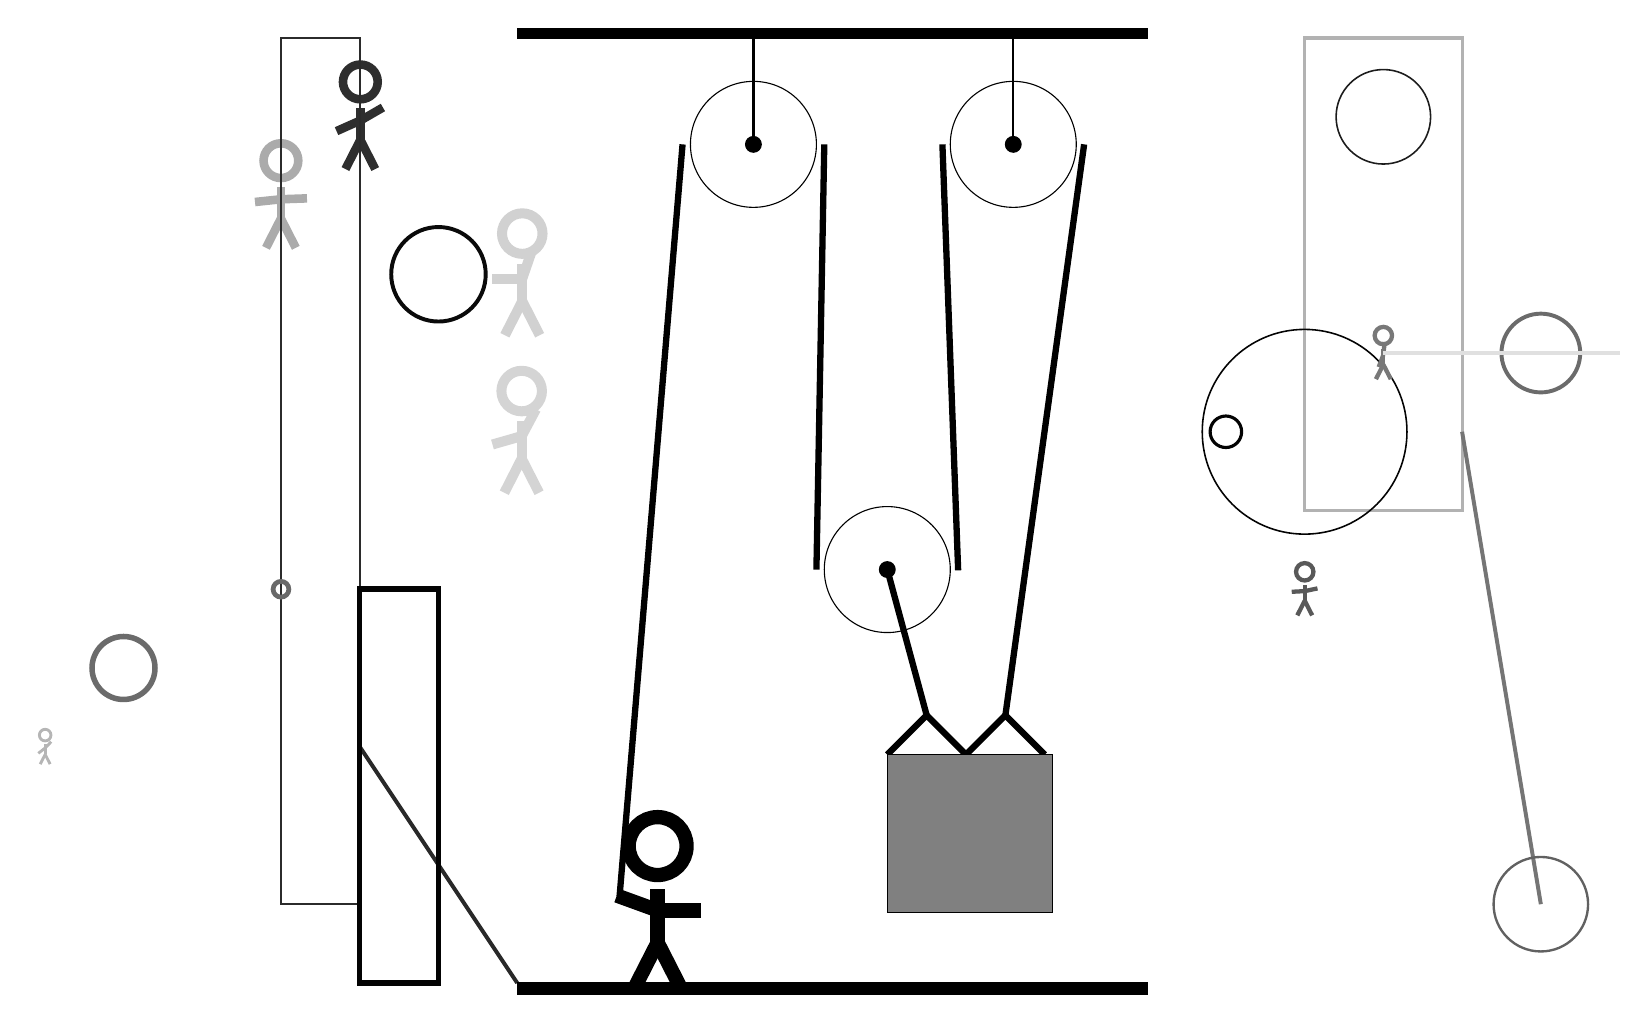
\begin{tikzpicture}
			%%%%% START %%%%%
			
			\draw[fill=black] (-2, 9) rectangle (6, 9.125);
			
			\draw (1, 7.65) circle (0.8);
			\draw[fill=black] (1, 7.65) circle (0.1);
			\draw[thick] (1, 7.65) -- (1, 9);
			
			\draw (4.3, 7.65) circle (0.8);
			\draw[fill=black] (4.3, 7.65) circle (0.1);
			\draw[thick] (4.3, 7.65) -- (4.3, 9);
			
			\draw (2.7, 2.25) circle (0.8);
			\draw[fill=black] (2.7, 2.25) circle (0.1);
			
			\draw[line width=0.8mm]  (2.7, -0.1) -- (3.2, 0.4) -- (3.7, -0.1) -- (4.2, 0.4) -- (4.7, -0.1);
			\draw[fill=black!50] (2.7, -0.1) rectangle (4.8, -2.1);
			
			\draw[line width=0.8mm](-0.7, -1.9) -- (0.1, 7.65);
			\centerarc[line width=0.8mm](1, 7.65)(0:180:0.9);
			\draw[line width=0.8mm](1.9, 7.65) -- (1.8, 2.25);
			\centerarc[line width=0.8mm](2.7, 2.25)(180:370:0.9);
			\draw[line width=0.8mm] (3.6, 2.24) -- (3.4, 7.65);
			\centerarc[line width=0.8mm](4.3, 7.65)(0:180:0.9);
			\draw[line width=0.8mm](4.2, 0.4) -- (5.2, 7.65);
			\draw[line width=0.8mm] (3.2, 0.4) -- (2.7, 2.25);
			
			\draw[line width=0.4mm, color=black!30] (8, 9) rectangle (10, 3);
			
			\draw [line width=0.2mm, color=black!99](8, 4) circle (1.3);
			\draw[line width=0.5mm, color=black!54](10, 4) -- (11, -2);
			\draw [line width=0.4mm, color=black!99](7, 4) circle (0.2);
			\node[line width=0.5mm, color=black!33] at (-5, 7) {\Strichmaxerl[6][6][2]};
			
			\draw [line width=0.3mm, color=black!62](11, -2) circle (0.6);
			
			\draw [line width=0.7mm, color=black!58](-7, 1) circle (0.4);
			\node[line width=0.4mm, color=black!82] at (-4, 8) {\Strichmaxerl[6][24][30]};
			\node[line width=0.7mm, color=black!18] at (-2, 6) {\Strichmaxerl[7][0][71]};
			\node[line width=0.6mm, color=black!53] at (9, 5) {\Strichmaxerl[3][69][84]};
			
			\draw[line width=0.3mm, color=black!83] (-4, 9) rectangle (-5, -2);
			\draw [line width=0.5mm, color=black!58](11, 5) circle (0.5);
			\draw [line width=0.2mm, color=black!89](9, 8) circle (0.6);
			\node[line width=0.5mm, color=black!17] at (-2, 4) {\Strichmaxerl[7][16][62]};
			\draw[line width=0.5mm, color=black!12](9, 5) -- (12, 5);
			\draw [line width=0.5mm, color=black!96](-3, 6) circle (0.6);
			\node[line width=0.6mm, color=black!65] at (8, 2) {\Strichmaxerl[3][3][12]};
			\draw [line width=0.6mm, color=black!59](-5, 2) circle (0.1);
			\node[line width=0.4mm, color=black!29] at (-8, 0) {\Strichmaxerl[2][38][46]};
			\draw[line width=0.5mm, color=black!84](-4, 0) -- (-2, -3);
			\draw[line width=0.7mm, color=black!99] (-4, 2) rectangle (-3, -3);
			
			\node at (-0.2, -2) {\Strichmaxerl[10][-20][0]};
			
			\draw[fill=black] (-2, -3) rectangle (6, -3.15);
			
			%%%%% END %%%%%
		\end{tikzpicture}
	\end{figure}	
\end{document}